\documentclass[11pt]{article}
\usepackage{../EllioStyle}

\title{Homework 0}
\author{Elliott Pryor}
\date{21 Aug 2020}


\begin{document}
\maketitle

\problem{1}
\begin{enumerate}[1.]
	\item What is polymorphism? Provide an example using source code
	\item What is inheritance? Describe the differences between public vs private inheritance
	\item What is encapsulation?
	\item What is the difference between static vs dynamic binding?
\end{enumerate}
\hrule

\begin{enumerate}[1.]
	\item Polymorphism is changing the function of a method in a parent class via inheritance. Figure \ref{fig:polymorph} shows a very simple example of polymorphism.	
	
	\begin{figure}[H]
	    \centering
	    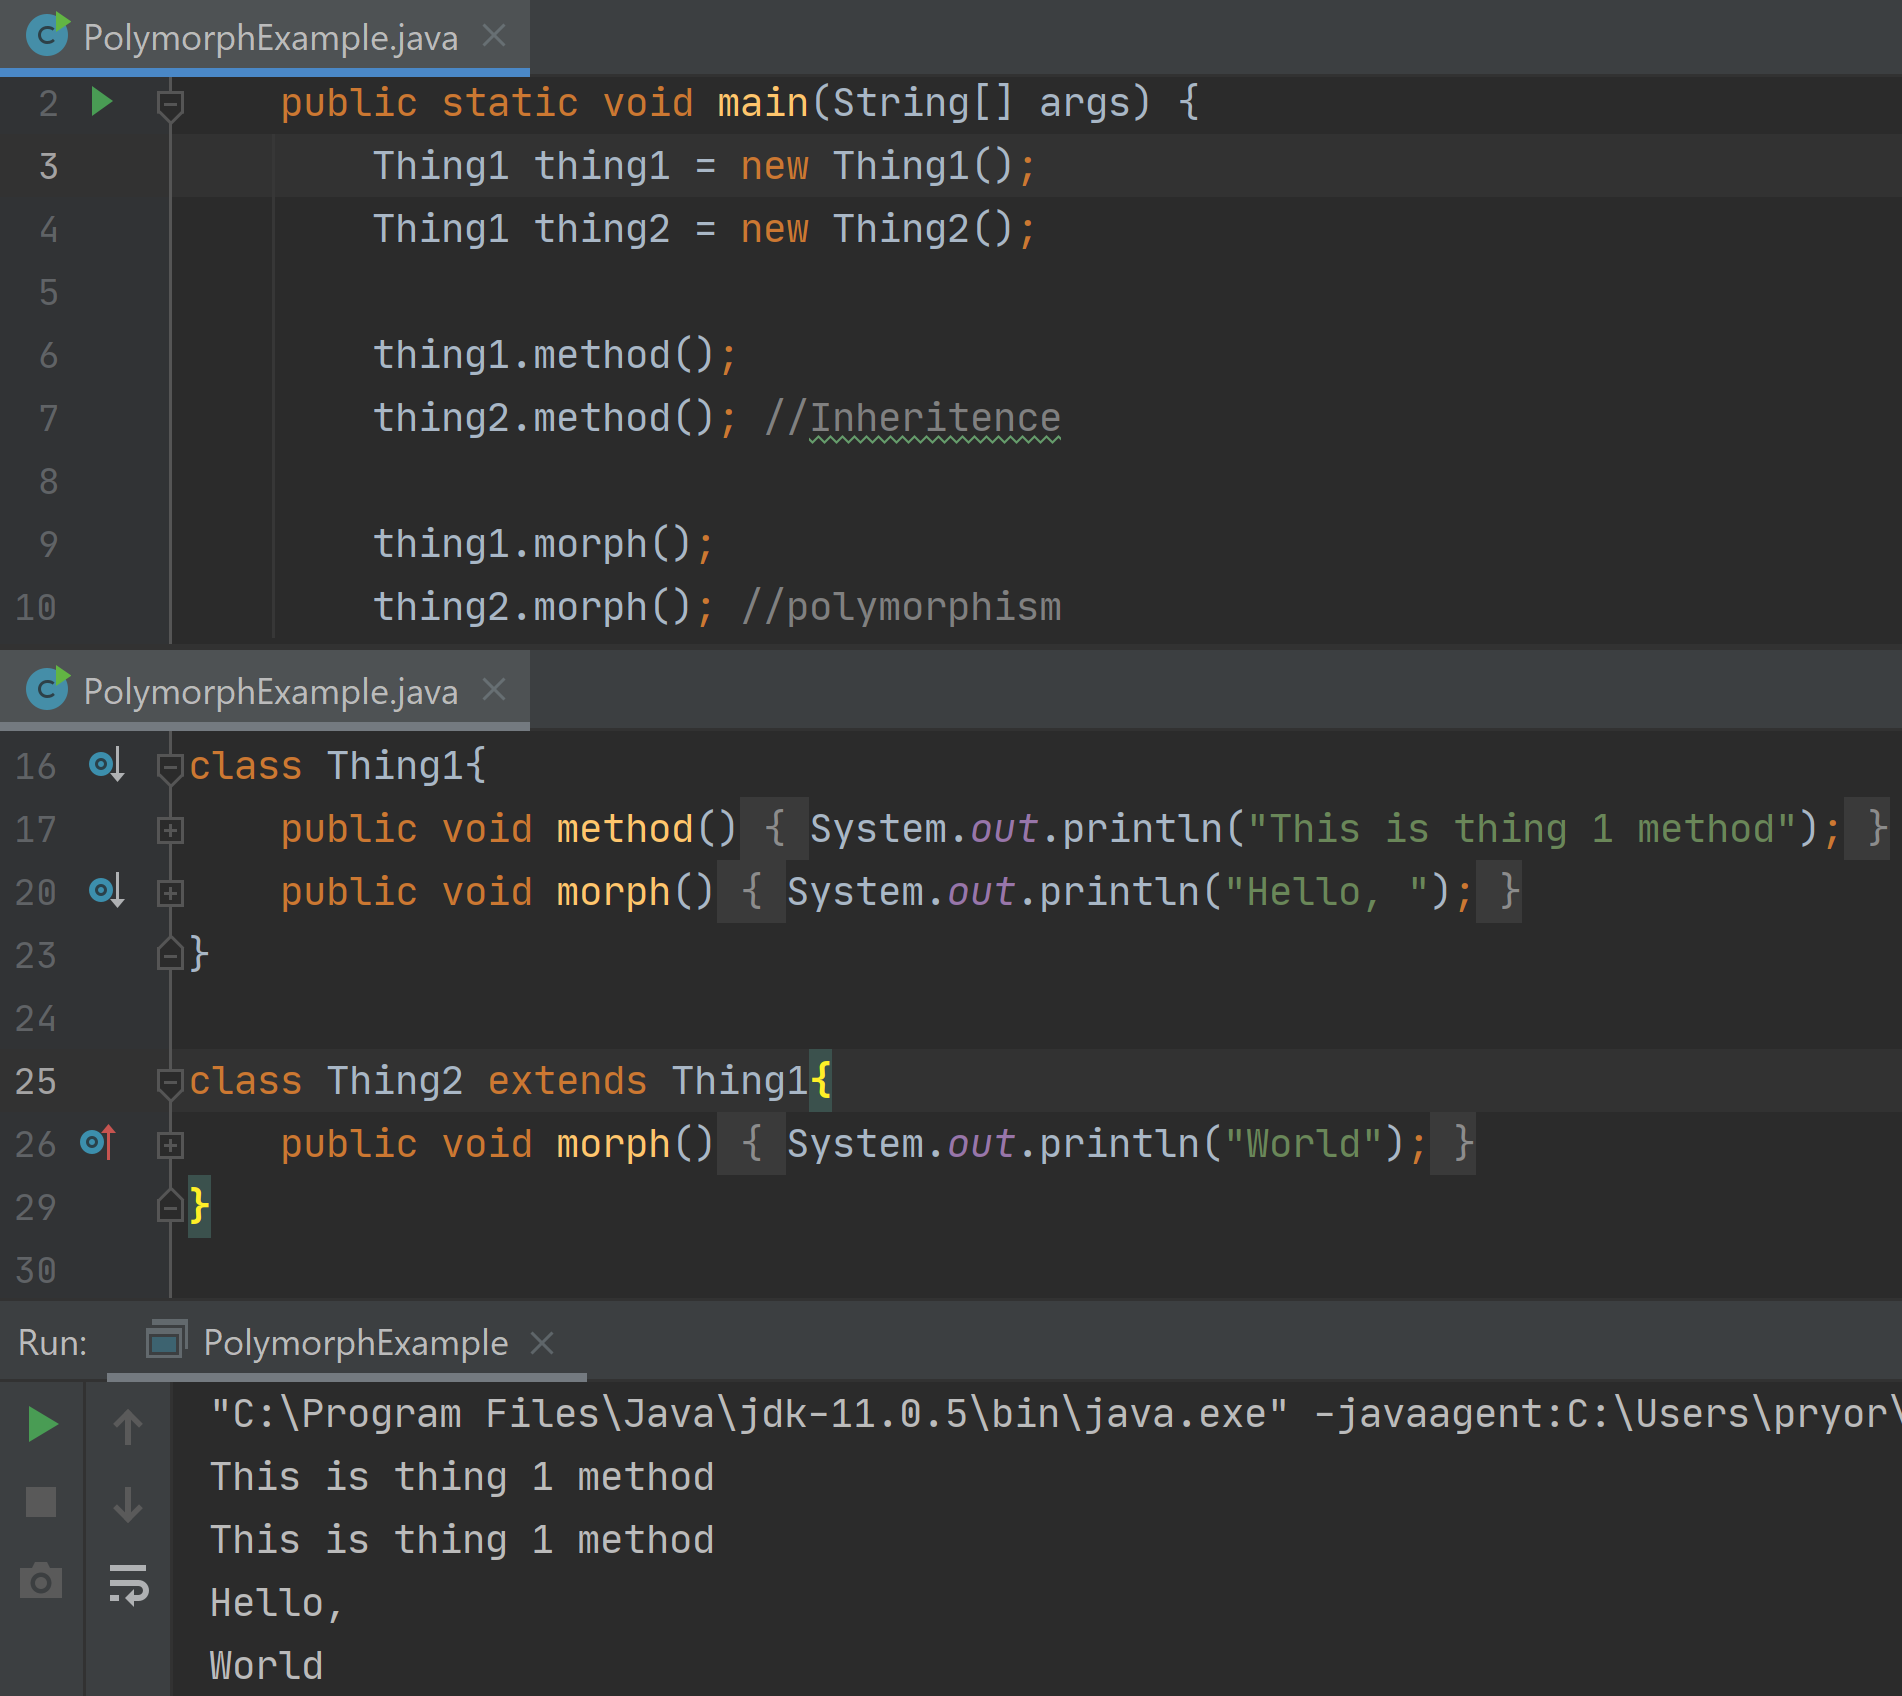
\includegraphics[width=0.5\textwidth]{../pictures/polymorph.png}
	    \caption{Example of polymorphism}
	    \label{fig:polymorph}
	\end{figure}
	
	\item Inheritance is when one class extends another and inherits the methods and variables from the parent class. The child class is a more specific type of the parent class. In public inheritance public methods in the parent class remain public methods in child class, but in private inheritance public methods in the parent class become private methods in the child class. In figure \ref{fig:polymorph} Thing1 is the parent class and Thing2 is the child class.
	\item Encapsulation is the restriction of access to a method or variable within a class. This limits unwanted access and can help protect functionality. A common example is the use of getters and setters for encapsulated variables. 
	\item Static binding is fixed and can't be changed (static). This would be done at compile-time, and cannot be overriden. Dynamic binding is loose and done during run-time. Dynamically bound methods can be changed during runtime (inheritance) \cite{singh_2013}
\end{enumerate}


\problem{2}
\begin{enumerate}[i.]
	\item Provide a definition for a prescribed lifecycle, and name two types of prescribed lifecycles
	\item For each type provide an example (i.e. a use case)
\end{enumerate}
\hrule

\begin{enumerate}[i.]
	\item A prescribed lifecycle is a processes of development. It outlines a methodology for how a piece of software can go from an idea to deployment. One example is the waterfal model, another example is the evolutionary model.
	\item The waterfall model is used for slow development projects. For example an operating system, we do not want a lot of changes, but instead go from design to deployment in one single chain. The evolutionary model is a cycle. It goes from design to deployment back to design very fast, so is good for prototyping. 
\end{enumerate}



\problem{3}

What does low coupling and high cohesion mean?
\hrule

Coupling is the amount of interdependence between modules. Low coupling is preferred because it means that modules can be changed without much influence to the rest of the program. 

Cohesion is how alike processes are within a module. If they all serve a common goal this leads to high cohesion as they are very alike and united. If a module has a more un-related subroutine this leads to low cohesion.
\cite{post,geeks}


\bibliographystyle{plainurl}
\bibliography{refs}



% refs
% vv dynamic vs static binding
% https://beginnersbook.com/2013/04/java-static-dynamic-binding/#:~:text=Static%20binding%20happens%20at%20compile,these%20methods%20cannot%20be%20overridden.&text=The%20binding%20of%20overloaded%20methods,of%20overridden%20methods%20is%20dynamic.

\end{document}